\documentclass[../root]{subfiles}
\graphicspath{{_images/}{../_images/}}


\begin{document}

    \chapter{Minimum wages and the labor market effects of immigration}

    \begin{shortsummary}
        \begin{itemize}
            \item \authoryear{Ed2019}
            \item \RQ{How minimum wage affect the impact of immigration?}
            \item \answer{Empirical analysis using the standard panel estimation and the difference-in-difference estimation.}
            \item \result{Higher minimmum wage reduce immigration negative impact especially low-skilled workers}
        \end{itemize}
    \end{shortsummary}

    \section{Introduction}
    \begin{itemize}
        \item Some of the recent studies found the immigration has significant negative effect because of labor supply shock. (e.g. Borjas 2003,Dustmann et.al 2016)
        \item Institution such as wage rigidity may prevent wages or employment to adjustment. 
        \item By using spatial correlation labor outcomes and measures of immigration, the early investigation could lead to misleading interpretations. 
    \end{itemize}
    The main contribution of this paper is to investigate the role of labor market institution.

    This paper conduct Empirical analysis to investigate the role of labor market institution, especially minimum wages.
    %もうちょっとイントロを考える
    
    The successive rises in the federal minimum wage between 2007 and 2010(from \$5.15 to \$7.25) \\
    The state's effective minimum wage(EMW) is equal to the higher one of the state-specific minimum wage(SMW) or the federal minimum wage(FMW).
    \begin{align*}
        EMW_{st}=Max(SMW_t, FMW_t)
    \end{align*}

    This paper conduct panel panel data estimation and DiD estimation using these data. 

    {\bf Instrument strategy}
    \begin{itemize}
        \item The number of immigrants and states effective minimum wage may be biased.
        \begin{itemize}
            \item This paper use the 1980 distribution of immigrants as instrument (Altomji and Card 1991) 
            \item This paper use the federal minimum wage as instrument(Baskaya and Rubinstein 2012)
        \end{itemize}
    \end{itemize}
    
    {\bf Results}
    \begin{itemize}
        \item The immigration impact for native's labor market outcomes is more negative in low-skilled workers.
        \item The high minimum wage reduce negative impact in native's outcome.  
    \end{itemize}

    \section{Theoretical framework}
    \begin{figure}[h]
        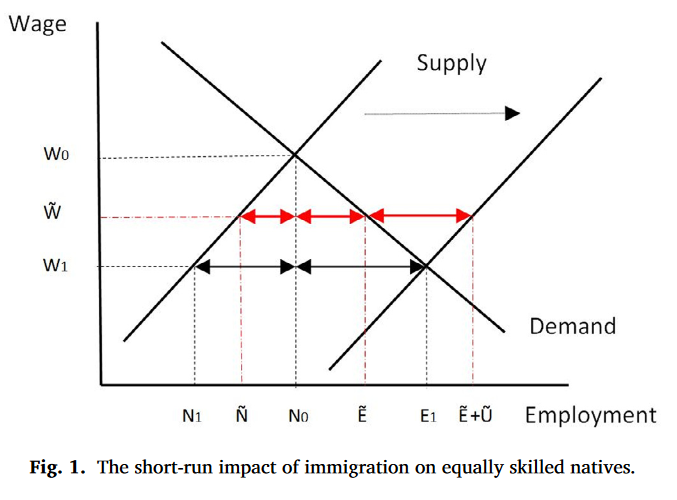
\includegraphics[width=12cm]{0612sugiyama/figure1.png}
    \end{figure}

    First equilibrium is $N_0$ and immigrants' labor supply  is added to $N_0$ and next equilibrium is $E_1$ when immigration  occur. \\
    In this case, wage is $w_1$ and some natives find it profitable stop working. \\

    If there is minimum wage ($W_1 < \tilde{W} < W_0$), there is some involuntary unemployment($\tilde{U}$).

    \begin{itemize}
        \item In the competitive case: $\partial W/ \partial M \equiv \eta_W <0$ and $\partial N / \partial M \equiv \eta_N <0$, where $\eta_W$ and $\eta_N$ denote the wage and native employment response to immigration, respectively.
        \item In the case of binding minimum wage: the negative effect of immigration on native labor outcomes smaller than in the competitive case.  $ \partial \eta_W/ \partial \tilde{W} >0$ and $\partial \eta_N / \partial \tilde{W} >0$.
    \end{itemize}

    If the participation rate is strongly responsive to a decline in wages, immigration will mainly increase inactivity $I$.
    Alternatively, a lower wage may not lead to increased inactivity if te participation rate is insensitive to wage changes. \\
    So, the response of inactivity is unobvious and the empirical section of this study will study these responses of by using two measures of natives' employment: as a share of the labor force, $N/(N+U)$ ; and as a share of the working age population, $N/(N+U+I)$.
    It is theoretically unclear whether a adjustment higher minimum wage will favor through unemployment or inactivity.
    

    \section{Data and empirical methodology}
    This paper exploit annual data from 2000-2013. \\
    Two sources of data:
    \begin{itemize}
        \item the Public Use Microdata Sample of the Census for the year 2000.
        \item American Community Survey for the subsequence years.
    \end{itemize}

    For weekly and hourly earnings are deflated to real 1999 dollars - this paper convert dollar amounts to 1999 dollars by using the consumer price index adjustment factors on the IPUMS website.
    This paper  divide people into the categories "employed", "unemployed", and "not in the labor force" to compute the employment rate.

    The immigrant supply shock experienced in a particular  skill-cell $i$ in states $s$ at year $t$ is measured by $p_{ist}$:
    \begin{align}
        p_{ist}=\frac{M_{ist}}{N_{ist}+M_{ist}}
    \end{align}

    All minimum wage data used in this study one directly taken from the U.S. Department of Labor.
    \begin{figure}[h]
        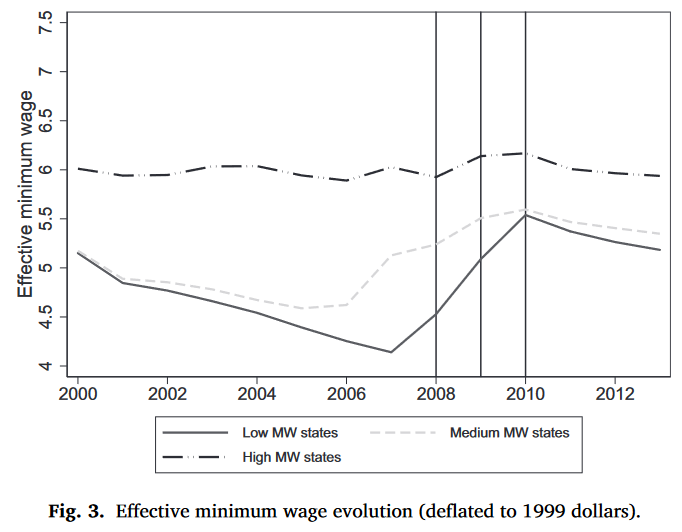
\includegraphics[width=12cm]{0612sugiyama/figure3.png}
    \end{figure}
    Figure 3 graph the evolution of the effective minimum wage for the there group of states. \\
    The there groups as follow:
    \begin{itemize}
        \item high minimum wage group:the states' EMW always higher than FMW(N=9)
        \item medium minimum wage group:the states' EMW sometimes higher than FMW(N=24)
        \item low minimum wage group: the state's EMW always lower than FMW(N=18)
    \end{itemize}

    This graph show real effective minimum wage was constant over the period at around \$6 for high MW group.
    The successive increases in the federal minimum wage only affected the low and medium wage is binding.

    This paper estimate the following mode to examine the impact of immigration on the  employment and wage of native workers.
    \begin{align}
        y_{ist}=\beta_0+\beta_1(p_{ist})+\beta_2(p_{ist} \times MW_{st}) +\delta_i + \delta_s + \delta_t + \delta_i \times \delta_s +\delta_i \times \delta_t +\delta_s \times \delta_t +\xi_{ist}, 
    \end{align} 
    where $\delta$ is fixed effect and outcomes are
    \begin{itemize}
        \item the mean log weekly wage
        \item the mean log hourly wage
        \item the mean log employment as share of population
        \item the mean log employment as share of the labor force
    \end{itemize}

    $\beta_1$ is likely very likely to be upward bias since immigrants are attracted mostly to places when wages and employment are high.
    
    {\bf IV strategy} \\
    To address this issue, this paper conduct an instrument variable approach following Altonji and Card(1991).

    This paper will use to build instrument the 1980 distribution of immigrants from a given country $c$ for a given skill group $i$ a cross U.S. states $s$ to allocate the new waves at immigrants from that skill-country group across states.
    
    Instrument $\hat{p_{ist}}$ is computed as follow:
    \begin{align}
        \hat{p_{ist}} =\hat{M}_{ist}/ (\hat{N}_{ist} +\hat{M}_{ist}),
    \end{align}
    where, 
    \begin{align}
        \hat{M}_{ist}=\sum_c\frac{M^c_{is}(1980)}{M^c_i(1980)} \times M^c_{i}(t)
    \end{align}
    and,
    \begin{align}
        \hat{N}_{ist}=\frac{N_{is}(1980)}{N_i(1980)} \times N_i(t)
    \end{align}

    If the determination of the state effective minimum wages has endogeneity, $\hat{\beta_2}$ is biased upward or downward.
    This paper use the federal minimum wage to instrument state's minimum wages, because (i) a change in the  federal minimum wage tend to be exogenous to local labor market conditions and (ii)  has differential effect on the effective wages across states. \\

    {\bf difference-in-difference strategy} \\
    As in show Fig.3, "low minimum wage" states were affected changing federal minimum wage and "high minimum wage" states' minimum wages were constant around $\$$6. \\
    This paper's Different-in-different (DiD) strategy compares the estimated effect of immigration before and after the policy changes in low- v. high minimum wage states.

    Changing federal minimum wage affect only treated group("low minimum wage").

    The DiD estimator of the differential labor market impact of immigration induced by the policy change at time $t$ can be defined as:

    \begin{align}
        \mathbb{E}[\hat{\beta}^{post}_1 - \hat{\beta}^{pre}_1|X, Treated =1] -\mathbb{E}[\hat{\beta}^{post}_1 - \hat{\beta}^{pre}_1|X, Treated =0], 
    \end{align}

    and this paper expect above effect is positive. 

    The DiD regression expressed by :
    \begin{align}
        y_{ist}=&\lambda_0+\lambda_1(p_{ist})+\lambda_2(p_{ist} \cdot Treated_s)+\lambda_3(p_{ist} \cdot dt_{2008})+\lambda_4(p_{ist} \cdot dt_{2009}) \\ \nonumber
        &+\lambda_5(p_{ist} \cdot dt_{2011})+\lambda_6(p_{ist} \cdot Treated_s \cdot dt_{2008}) \\ \nonumber
        &+\lambda_7(p_{ist} \cdot Treated_s \cdot dt_{2009})+\lambda_8(p_{ist} \cdot Treated_s \cdot dt_{2010}) \\ \nonumber
        &+\delta_i + \delta_s + \delta_t + \delta_i \times \delta_s +\delta_i \times \delta_t +\delta_s \times \delta_t +\mu_{ist}, 
    \end{align}


    The key coefficients, $\lambda_6, \lambda_7, \lambda_8$ measure the DiD estimates of the policy interventions on the effects of immigration on $y_{ist}$ in the treated v. control groups.


    \section{Main results}
    {\bf OLS results} \\
    \begin{figure}[h]
        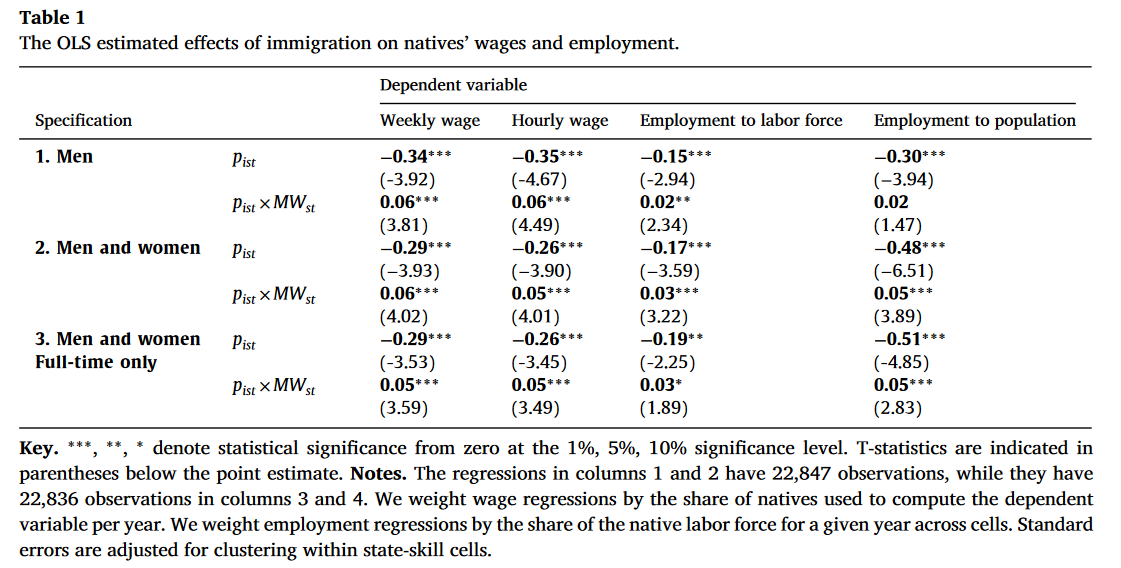
\includegraphics[width=12cm]{0612sugiyama/Table1.png}
    \end{figure}
    Table 1 show the OLS results.This paper weight wage regressions by the that of observations used to compute the mean wage per state-skill vell of time.

    \begin{itemize}
        \item Immigration had negative and significant effect on natives' wage.
        \item Minimum wage reduce the wage negative effect of immigration.
        \item From column 3 and 4, unemployment and inactivity were affected by immigration.
        \item From column 4, and row 1 and 2, women's labor supply is  more responsive to wage changes than men's labor supply of te extensive margin. 
        \item From the row 3, full-time workers' reservation wage are higher than part-time workers' one.
    \end{itemize}
    

    Using mean of the MW($\overline{MW}= 5.16 $), this paper estimate the total impact of immigration on native weekly wages as
    \begin{align*}
        -0.03&= \hat{\beta_1} + \hat{\beta_2} \times \overline{MW}_{st} \\
            &= -0.34+0.06 \times 5.16 
    \end{align*}
    As in Borjas(2003), wage elasticity for weekly earnings as 
    \begin{align*}
        -0.02 &= \mbox{total impact of immiration} \times (1-p_{ist})^2 \\
            &=-0.03 \times 0.68 
    \end{align*}

    As same way, the native's wage and employment elasticity w.r.t minimum wage is 0.04 and 0.01, respectively.
    
    
    \begin{figure}[h]
        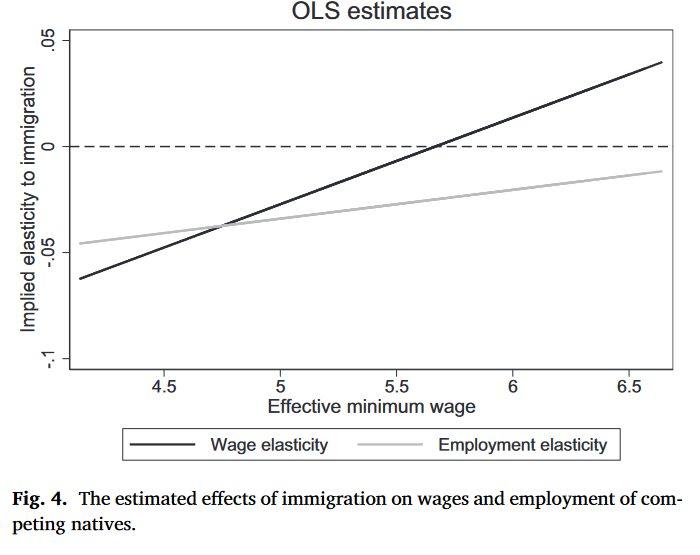
\includegraphics [width=12cm]{0612sugiyama/figure4.png}
    \end{figure}

    Fig 4 represent the relationship between elasticity and minimum wage.

    {\bf IV results} \\

    \begin{figure}[h]
        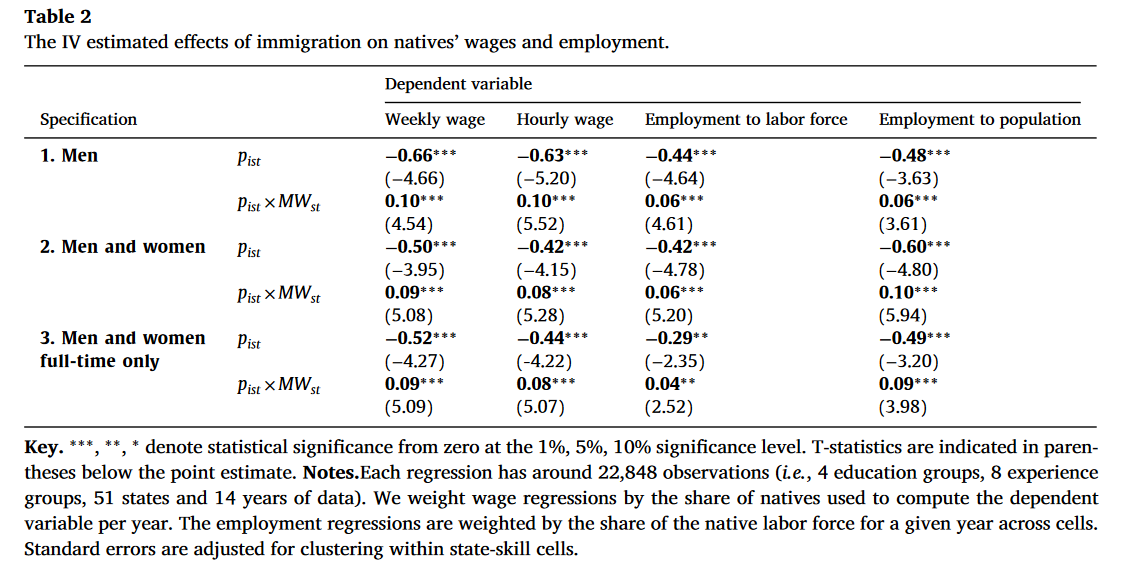
\includegraphics[width=12cm]{0612sugiyama/table2.png}
    \end{figure}

    Table 2 show immigrants IV results.

    \begin{itemize}
        \item IV results are consist with OLS results.
        \item Upper bias can be reduced by IV.
        \item The wage elasticity is -0.16
        \item The mean impact of immigration on the employment rate to labor force is around -0.09(OLS based is -0.03)
    \end{itemize}
    
    {\bf IV results for minimum wage}
    \begin{figure}[h]
        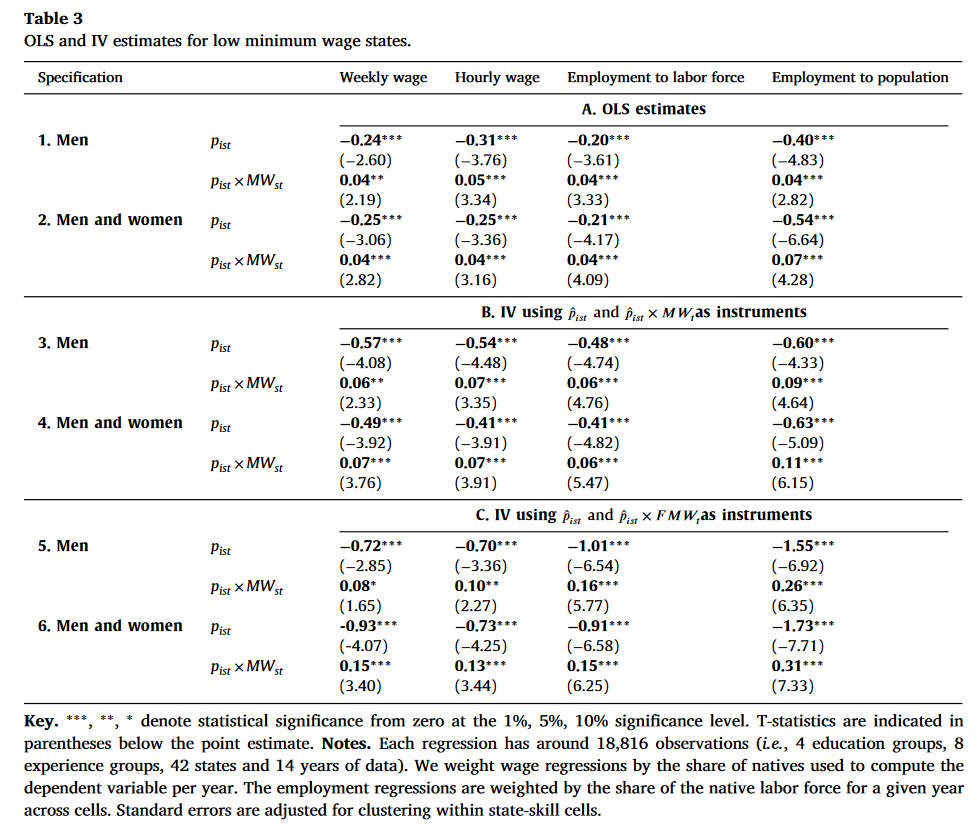
\includegraphics[width=12cm]{0612sugiyama/Table3.png}
    \end{figure}

    $MW_{st}$ are likely endogenous to state labor market condition such as a positive productivity condition or changing their labor market flexibility. So, this paper conduct IV estimation w.r.t minimum wage and table 3 show the results of IV estimation.
    These bias is unclear because positive productivity shock may induce upper bias and changing labor flexibility may induce downward bias.
    
    IV strategy is (i) excluding higher minimum state and (ii) instrumenting $MW_{st}$ by the federal for the remaining group of states.
    
    \begin{itemize}
        \item From panel A and B, we can check robust results of above.
        \item From panel C, minimum wage has downward bias for immigration impact.
        \item The negative relationship is heterogeneous w.r.t. the level of states' effective minimum wage.
        \item $\overline{MW}_{st}=4.98$ and the wage elasticity to immigration is -0.03 in panel A, -0.18 in panel B, and -0.22 in panel C
        \item The average employment to immigration is -0.001 in panel A, -0.12 in panel B, and -0.14 in panel C.   
    \end{itemize}

    {\bf The estimation focusing low-skilled workers}
    \begin{figure}[h]
        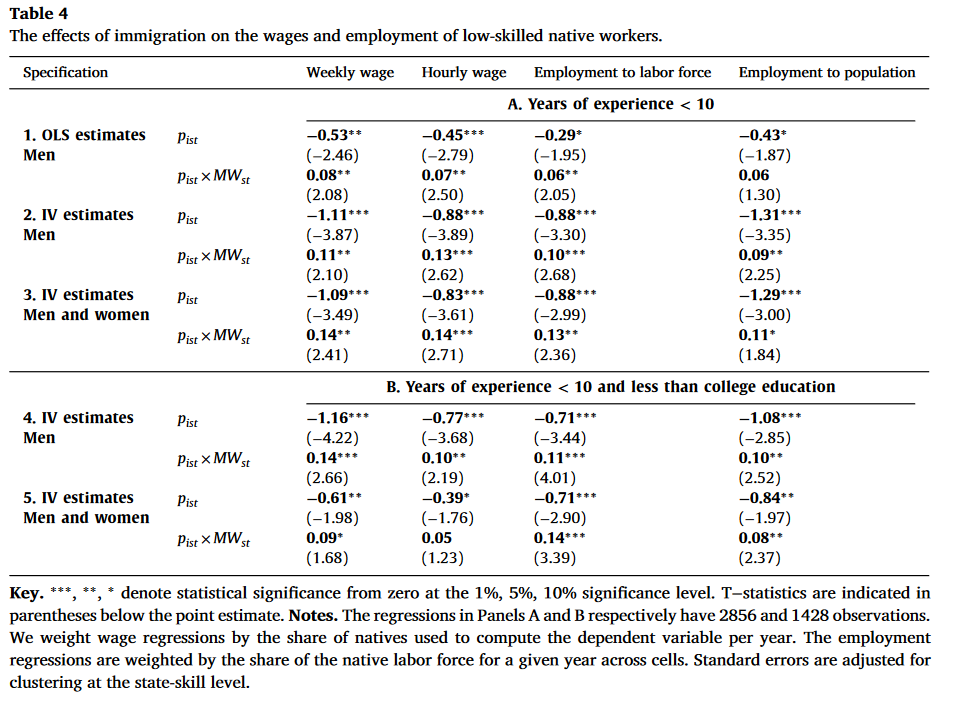
\includegraphics[width=12cm]{0612sugiyama/Table4.png}
    \end{figure}

    Table 4 show the estimation of focusing low-skilled workers.
    \begin{itemize}
        \item Low-skilled worker were affected more negative effect from the immigration impact.
        \item $\overline{MV}_{st}=5.16$ and from row 4,  the wage elasticity -0.3.
        \item From row 2 and 4, the employment elasticity log employment rate to labor force(log employment rate population) are respectively -0.25(-0.58) and (-0.10) -0.38.
        \item From row 2, \$ 1 increasing the minimum wage reduces the wage (employment) elasticity to immigration by 0.075(0.07).
    \end{itemize}
    
    {\bf Difference-in-difference estimation}
    \begin{figure}[h]
        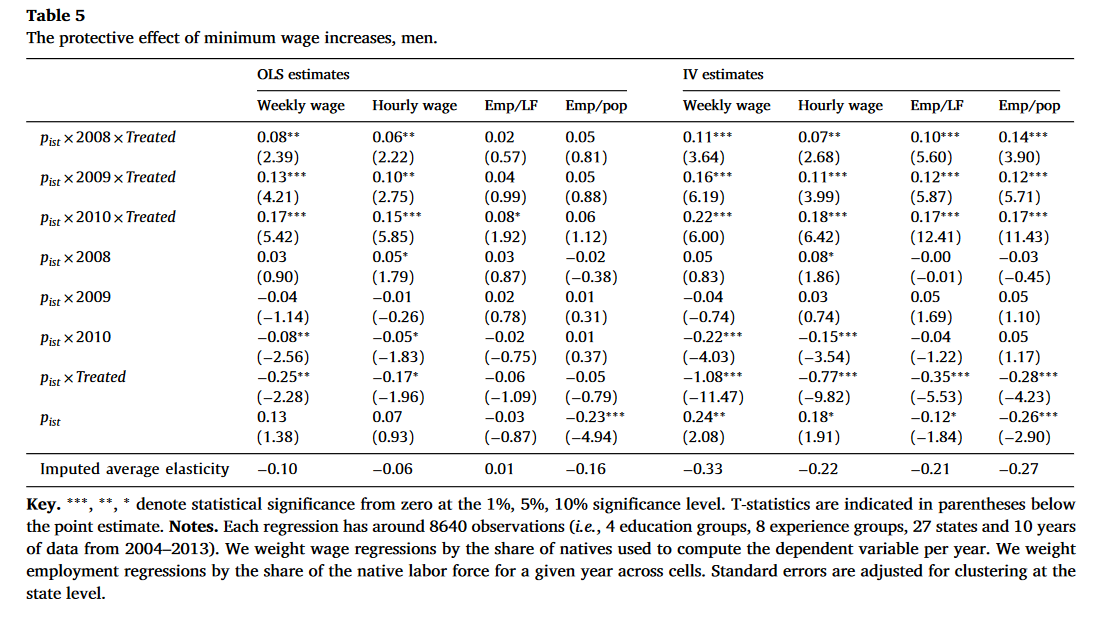
\includegraphics[width=12cm]{0612sugiyama/Table5.png}
    \end{figure}
    Table 5 provide OLS and IV estimation based on difference-in-difference for the sample of men.

    \begin{itemize}
        \item A rise in the federal minimum wags and employment of native workers who reside in states were the federal minimum is binding.
        \item The protective effect induced by the federal minimum rises ave been increasingly stronger.
    \end{itemize}

    The increasing protective effect relate to the increasing share of male native workers paid of minimum wage(from 7.4$\%$ in 2009 -10.7$\%$ in 2010) 


    \section{Conclusion}
    This paper conduct two empirical strategies (standard panel estimation and difference-in-difference estimation) to estimate the effect of minimum wage on the immigration impact.

    From the standard panel estimation;
    \begin{itemize}
        \item Immigration has negative effect on the native wages and employment outcomes of native workers.
        \item heterogeneous effect across U.S. states characterized by different levels of minimum wage. 
    \end{itemize}
    

    From the DiD estimation;
    \begin{itemize}
        \item The detrimental impact of immigration on natives' wages and employment has been mitigated in "treated" states.
    \end{itemize}

    From these results, this paper conclude high minimum wage protect native workers from immigration  impact.
    Higher minimum wage means high restrict for labor market and native unemployment or new immigrants have less across to employment.

    \biblio
    
    
\end{document}